%!TEX root = main.tex
\section{Introduction}

\subsection{Harmful Algal Blooms}
%%%%%%%%%%%%%%%%%%%%%%%%%%%%%%%%%%%%%%%%%%%
\begin{frame}{Harmful Algal Blooms}

\begin{columns}
	\column{0.5\textwidth}

	\begin{itemize}
		\item Explosive growth of microscopic algae and cyanobacteria
		\item Increase in primary productivity
		\item Toxin-producing genera
		\item Decrease biodiversity
		\item Anoxic environment
	\end{itemize}

	\column{0.5\textwidth}
	\begin{figure}
		\hspace*{-1cm}
		%\vspace*{-1cm}
		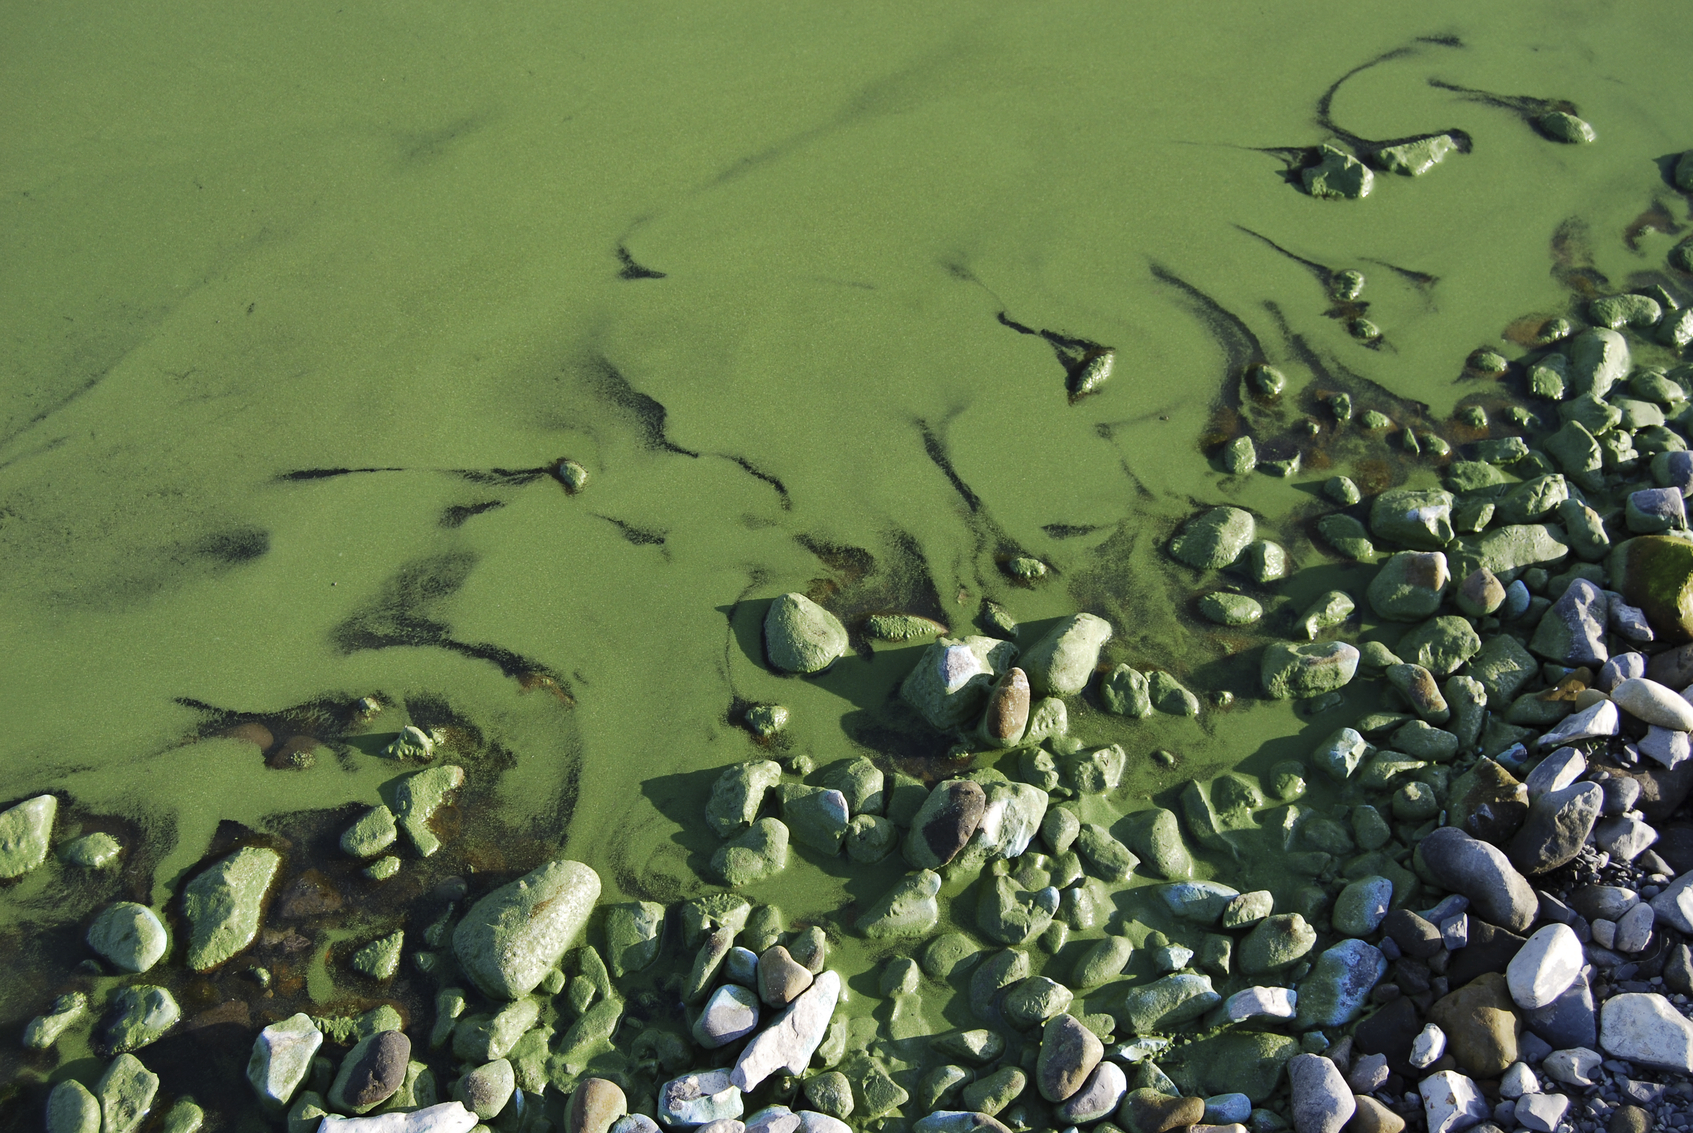
\includegraphics[width=2in,height=2in]{algal.jpg} \textsubscript{a}
		
	\end{figure}
\end{columns}
\footcitetext{[a]http://www.pme.com/wp-content/uploads/algal.jpg}
\end{frame}
%%%%%%%%%%%%%%%%%%%%%%%%%%%%%%%%%%%%%%%

\begin{frame}{Exposure Route}
	\begin{columns}
		\column{0.5\textwidth}
	\begin{itemize}
		\item Exacerbate from anthropogenic causes \textsubscript{a}
		\begin{itemize} 
			\item Some do naturally occur
		\item Worldwide issue
		\item Coastal environments
		\item Freshwater lakes
	\end{itemize}
\end{itemize}

	\begin{itemize}
		\item Direct contact
			\begin{itemize}
				\item Aerosols
				\item Ingestion
				\begin{itemize}
					\item Seafood/Fish 
					\item Drinking water
					\item Algal supplements
				\end{itemize}
			\end{itemize}
	\end{itemize}
	\column{0.5\textwidth}
	\begin{figure}
		\centering
		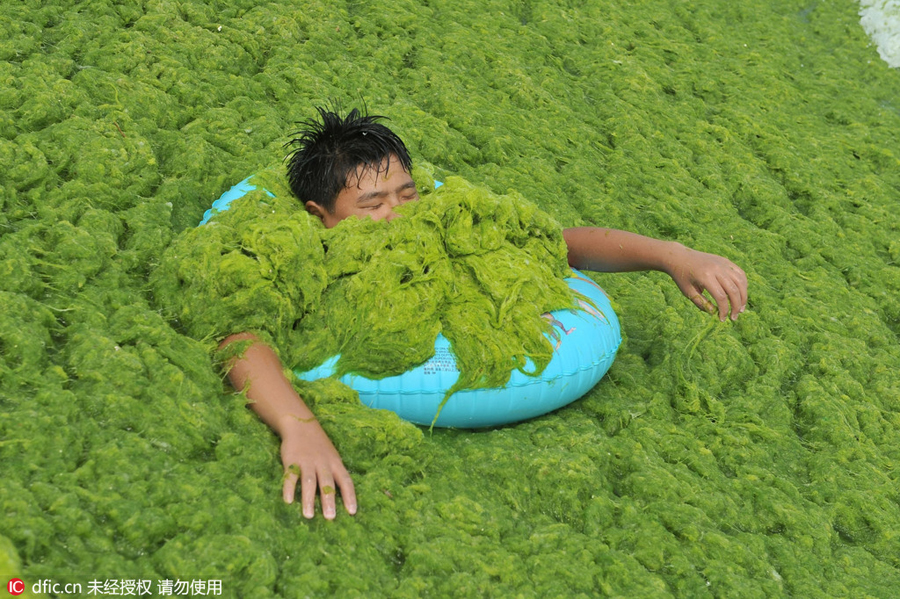
\includegraphics[width=2in]{swim.jpg} \textsuperscript{b}
		
	\end{figure}
\end{columns}
\footcitetext{[a], rastogi_cyanotoxin-microcystins:_2014}
\footcitetext{[b]https://www.ibtimes.co.uk/china-yellow-sea-turns-green-qingdao-beaches-are-covered-algae-photos-1509734}

\end{frame}
%%%%%%%%%%%%%%
\begin{frame}{Law and Regulation}
	\begin{columns}
		\column{0.5\textwidth}
	\begin{itemize}
		\item World Health Organization \textsuperscript{a}
		\item Safe Drinking Water Act \textsuperscript{b}  	
		\item Maximum Contaminant Level 
			\begin{itemize}
				\item Regulated and enforced
			\end{itemize}
		\item Contaminant Candidate List \textsuperscript{c} 
			\begin{itemize}
				\item ``More like guidelines''
			\end{itemize}
		\item Ambient Water Quality Criteria \textsuperscript{d}
	\end{itemize}

	\column{0.5\textwidth}
	\begin{figure}
		\centering
		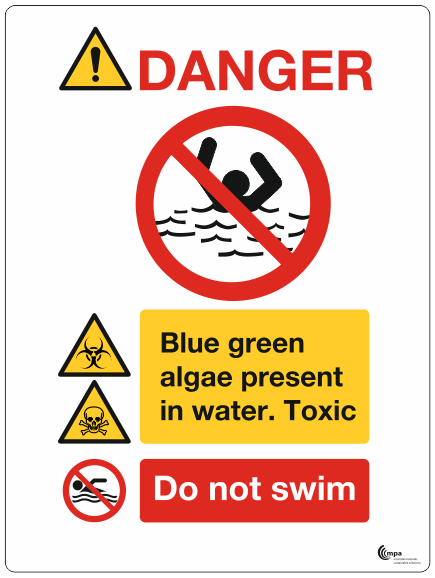
\includegraphics[scale=0.3]{warning.PNG}
	\end{figure}
	
	\end{columns}
	\footcitetext{[a], http://www.who.int/water/dwq/chemicals/cyanobactoxins.pdf}
	\footcitetext{[b], noauthor_guidelines_1998}
	\footcitetext{[c], usepa_drinking_2016}
	\footcitetext{[d], https://www.epa.gov/sites/production/files/monitoringRec.pdf}
\end{frame}
%%%%%%%%%%%%%%


\begin{frame}{Lake Erie 2014}
	\begin{figure}
		\centering
		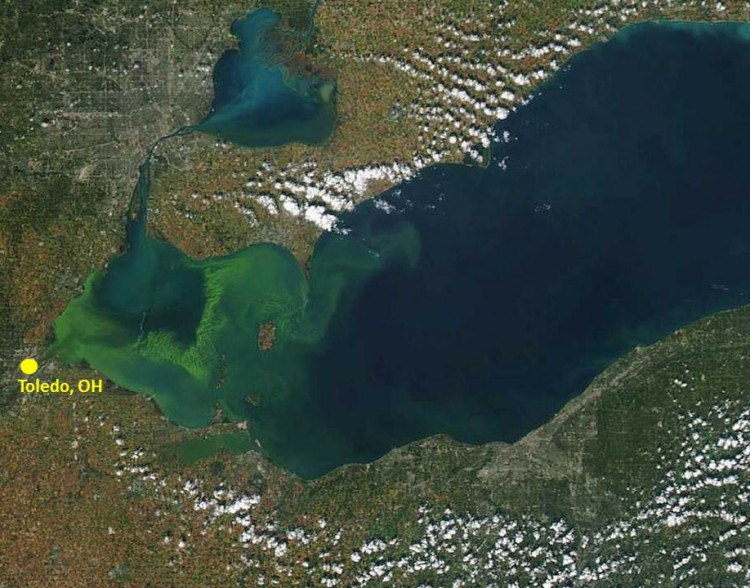
\includegraphics[scale=0.35]{erie.jpg}
	\end{figure}
\hrule
{\tiny cdn.coastalscience.noaa.gov}
\end{frame}
%%%%%%%%%%%%%%
\subsection{Cyanotoxins}
\begin{frame}{Cyanotoxins}

	\begin{itemize}
		\item Toxins
			\begin{itemize} 
				\item Microcystin and nodularin %\textsuperscript{1}
  				\item Cylindrospermopsin 
				\item Anatoxin 
				\item Saxitoxin 
				\item Produced nonribosomal polyketide synthase
			\end{itemize}
		\item Irritants
			\begin{itemize}
				\item Lipolysacharides \textsuperscript{a}
			\end{itemize}

	\end{itemize}
	\footcitetext{[a], moore_richard_cyanobacterial_1993}
\end{frame}
%%%%%%%%%%%%%%

\begin{frame}{Microcystin}

\begin{columns}
	\begin{column}{0.5\textwidth}

	\begin{itemize}
		\item Cyclic peptide
		\item Hepatoxin and carcinogenic
		\item Inhibits protein phosphatase
		\item Diverse structures 
		\item Intra-peritoneal LD\textsubscript{50} ranging from 25-150 $\mu$g/kg  \textsuperscript{a}
			\begin{itemize}
				\item Health Advisory (HA) of 4 $\mu$g/L over one day \textsuperscript{b}
			\end{itemize}
		\item Nonribosomally polyketide synthase (NRPS)
	\end{itemize}
	\end{column}
	\begin{column}{0.3\textwidth}
\begin{figure}[ht]
	\centering
	\hspace*{-1cm}
	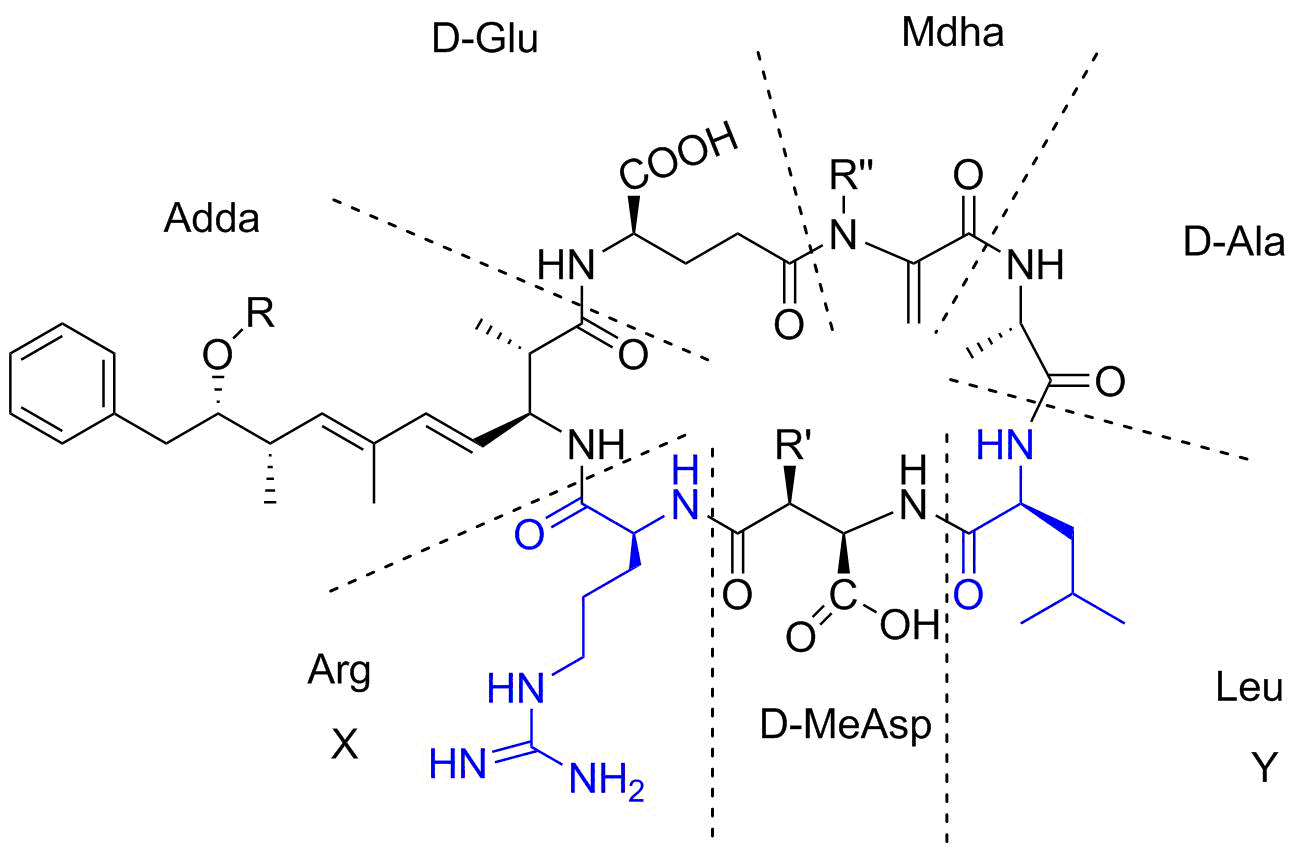
\includegraphics[width=2in, height=2.2in]{../figures/Microcystin-LR.png}
\end{figure}
	\end{column}
\end{columns}
\footcitetext{[a], dittmann_cyanobacterial_2012}
\footcitetext{[b], usepa_draft_2016}
\end{frame}
%%%%%%%%%%%%%%
\begin{frame}{Cylindrospermopsin}

\begin{columns}
	\column{0.5\textwidth}
	\begin{itemize}
		\item Polycyclic uracil derivative\textsuperscript{a} 
		\item Toxicity not fully understood\textsuperscript{b}
			\begin{itemize}
				\item Covalently binds to DNA/RNA 
				\item Inhibits protein synthesis %\textsuperscript{3} 
			\end{itemize}
		\item LD\textsubscript{50} of 150-200 $\mu$/kg over 5 days\textsuperscript{c}
			\begin{itemize}
				\item Health Advisory of 8 $\mu$g/L over one day\textsuperscript{d}
			\end{itemize}
	\end{itemize}
	\column{0.5\textwidth}
	\begin{figure}
		%\hspace*{-10cm}
		\centering
		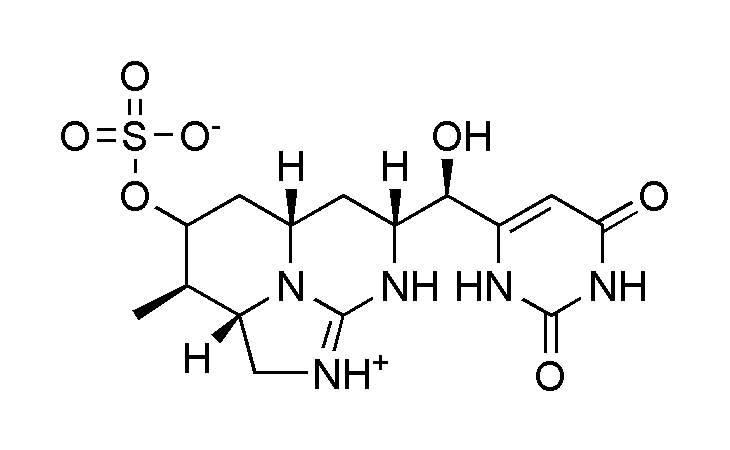
\includegraphics[width=2in]{cylindro.png}
	\end{figure}
\end{columns}
\footcitetext{[a], moreira_cylindrospermopsin:_2013}
\footcitetext{[b], kittler_1._2014}
\footcitetext{[c], shaw_cylindrospermopsin_2000}
\footcitetext{[d], usepa_draft_2016}
\end{frame}
%%%%%%%%%%%%%%
\begin{frame}{Anatoxin-a}
\begin{columns}
	\column{0.5\textwidth}
	\begin{itemize}
		\item Alkaloid 
		\item Known as Very Fast Death Factor \textsuperscript{a}
			\begin{itemize}
				\item Binds to acetylcholine receptor
				\item Paralysis 
				\item Respiratory failure
			\end{itemize}
		\item LD\textsubscript{50} of 300-375 $\mu$g/kg over 24 \textsuperscript{b}
	\end{itemize}
	\column{0.5\textwidth}
	\begin{figure}
		%\hspace*{-10cm}
		\centering
		
\includegraphics[width=2in]{anatoxin.png}
	\end{figure}
	\hspace*{-3cm}
\end{columns}
\footcitetext{[a], codd_cyanobacterial_1999}
\footcitetext{[b], shaw_cylindrospermopsin_2000}
\end{frame}
%%%%%%%%%%%%%%
\begin{frame}{Saxitoxin}
\begin{columns}
	\column{0.5\textwidth}
	\begin{itemize}
		\item Neurotoxin  
		\item Sodium channel blocker
		\item Paralytic shellfish poisoning
			\begin{itemize}
				\item Respiratory failure 
				\item Mouth-to-mouth resuscitation 
			\end{itemize}
		\item LD\textsubscript{50} of 2-10$\mu$g/kg over 24 h 
	\end{itemize}
	\column{0.5\textwidth}
	\begin{figure}
		%\hspace*{-10cm}
		\centering
		
\includegraphics[width=2in]{saxitoxin.png}
	\end{figure}
\end{columns}
\footcitetext{saoudi_management_2017}
\end{frame}
%%%%%%%%%%%%%%
\subsection{Survey Objectives}
\begin{frame}{Objectives}
	\begin{itemize}
		\item Investigate possible drivers of Harmful Algal Blooms 
		\item Evaluate a new monitoring technique
		\item Do lake's with heavy urbanized watershed have an association with HABs? 
	\end{itemize}
\end{frame}
%%%%%%%%%%%%%%
\section{Survey Methods}
\subsection{Sampling}
\begin{frame}{Surveyed Lakes}

\begin{figure}
	\centering
	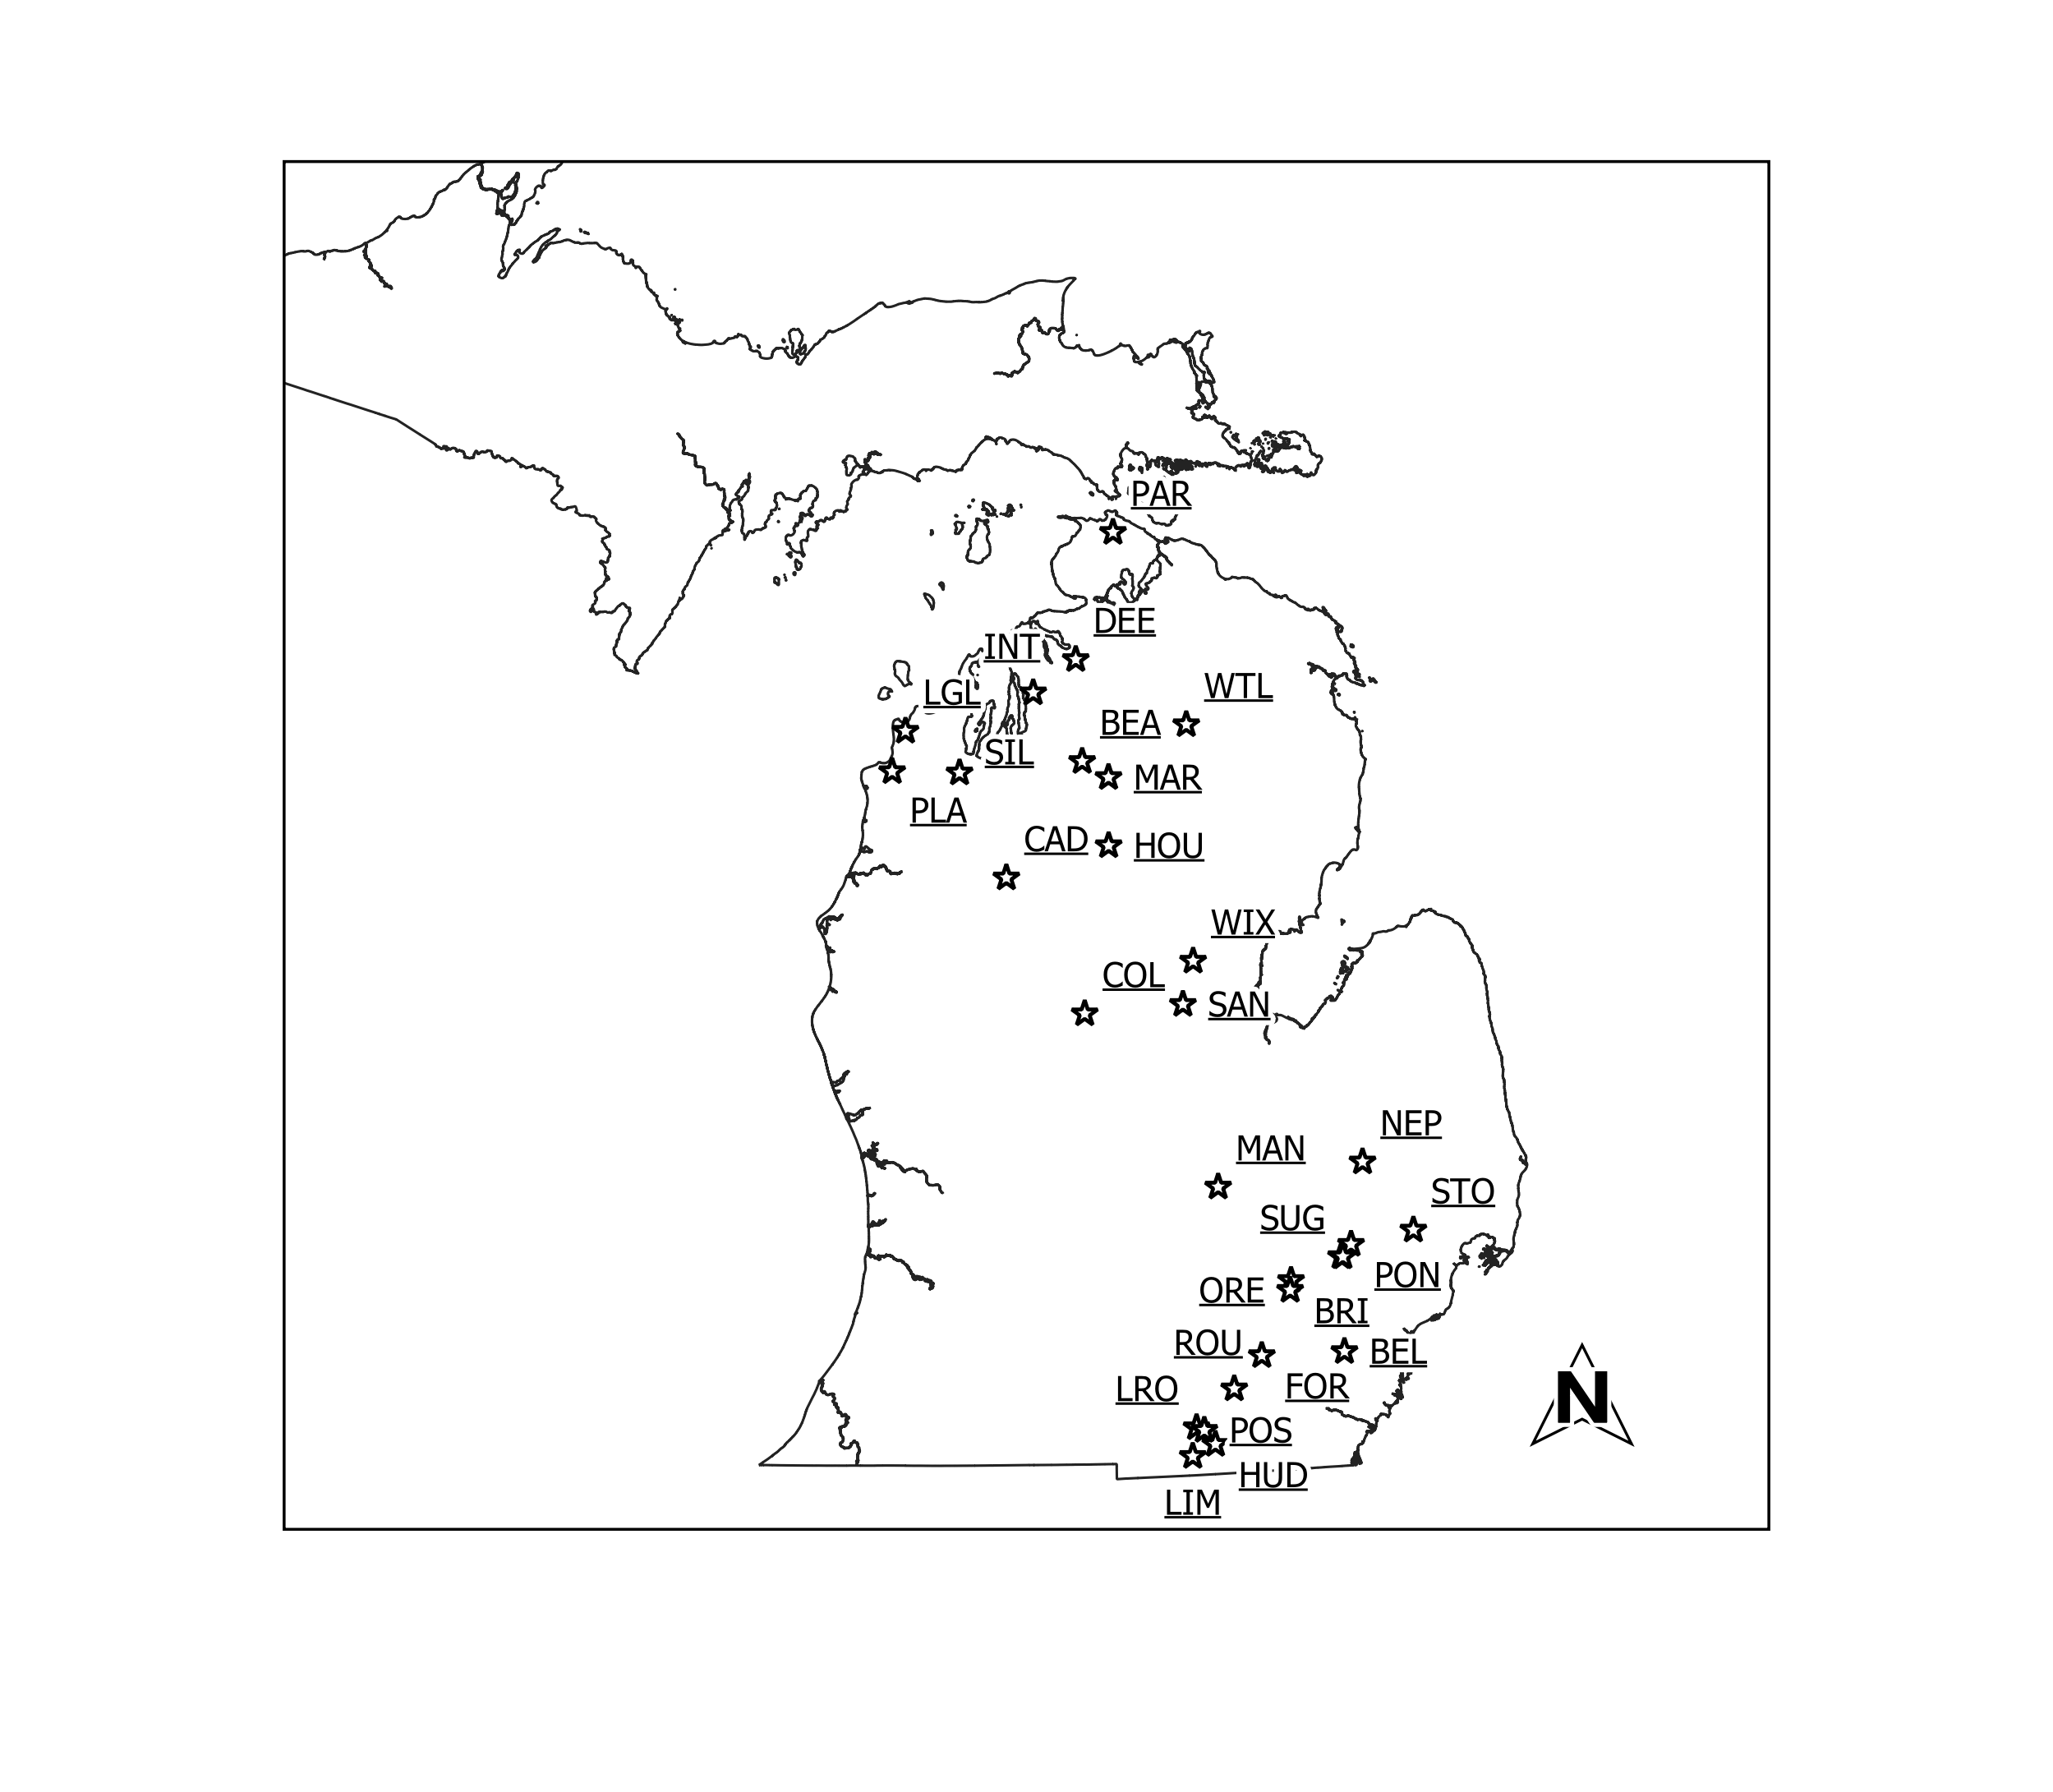
\includegraphics[width=0.8\textwidth,height=\textheight]{../figures/Overview.png}
	\caption{Sampled Lakes}
\end{figure}

\end{frame}

%%%%%%%%%%%%%%%%%%%%%%%%%%
\begin{frame}{Water Sampling}

	\begin{itemize}
		\item Sampled each lake once a month
		\item Collected water grab samples
			\begin{itemize}
				\item Waded in towards the center of the lake until water reaches waist height
				\item Water samples are taken roughly 10-20cm below the surface
			\end{itemize}
		\item Quickly transported back
		\item Analyzed ASAP
	\end{itemize}

\end{frame}
%%%%%%%%%%%%%%%%%%%%%%%%%%%%%
\begin{frame}
	\frametitle{Sampler}
\begin{columns}
	\column{0.5\textwidth}
	\begin{itemize}
		\item 3 PVC plates for collecting Zebra mussels (\emph{Dreissena polymorpha})
		\item Slotted PVC tube to hold SPATT 
		\item Installed on riparian owner's dock or on labeled floats  
		\item From July 2017 to October 2017
		\item Temperature/Light loggers 
		\item Mature Zebra mussels are collected in October
	\end{itemize}
	\column{0.5\textwidth}
	\begin{figure}
		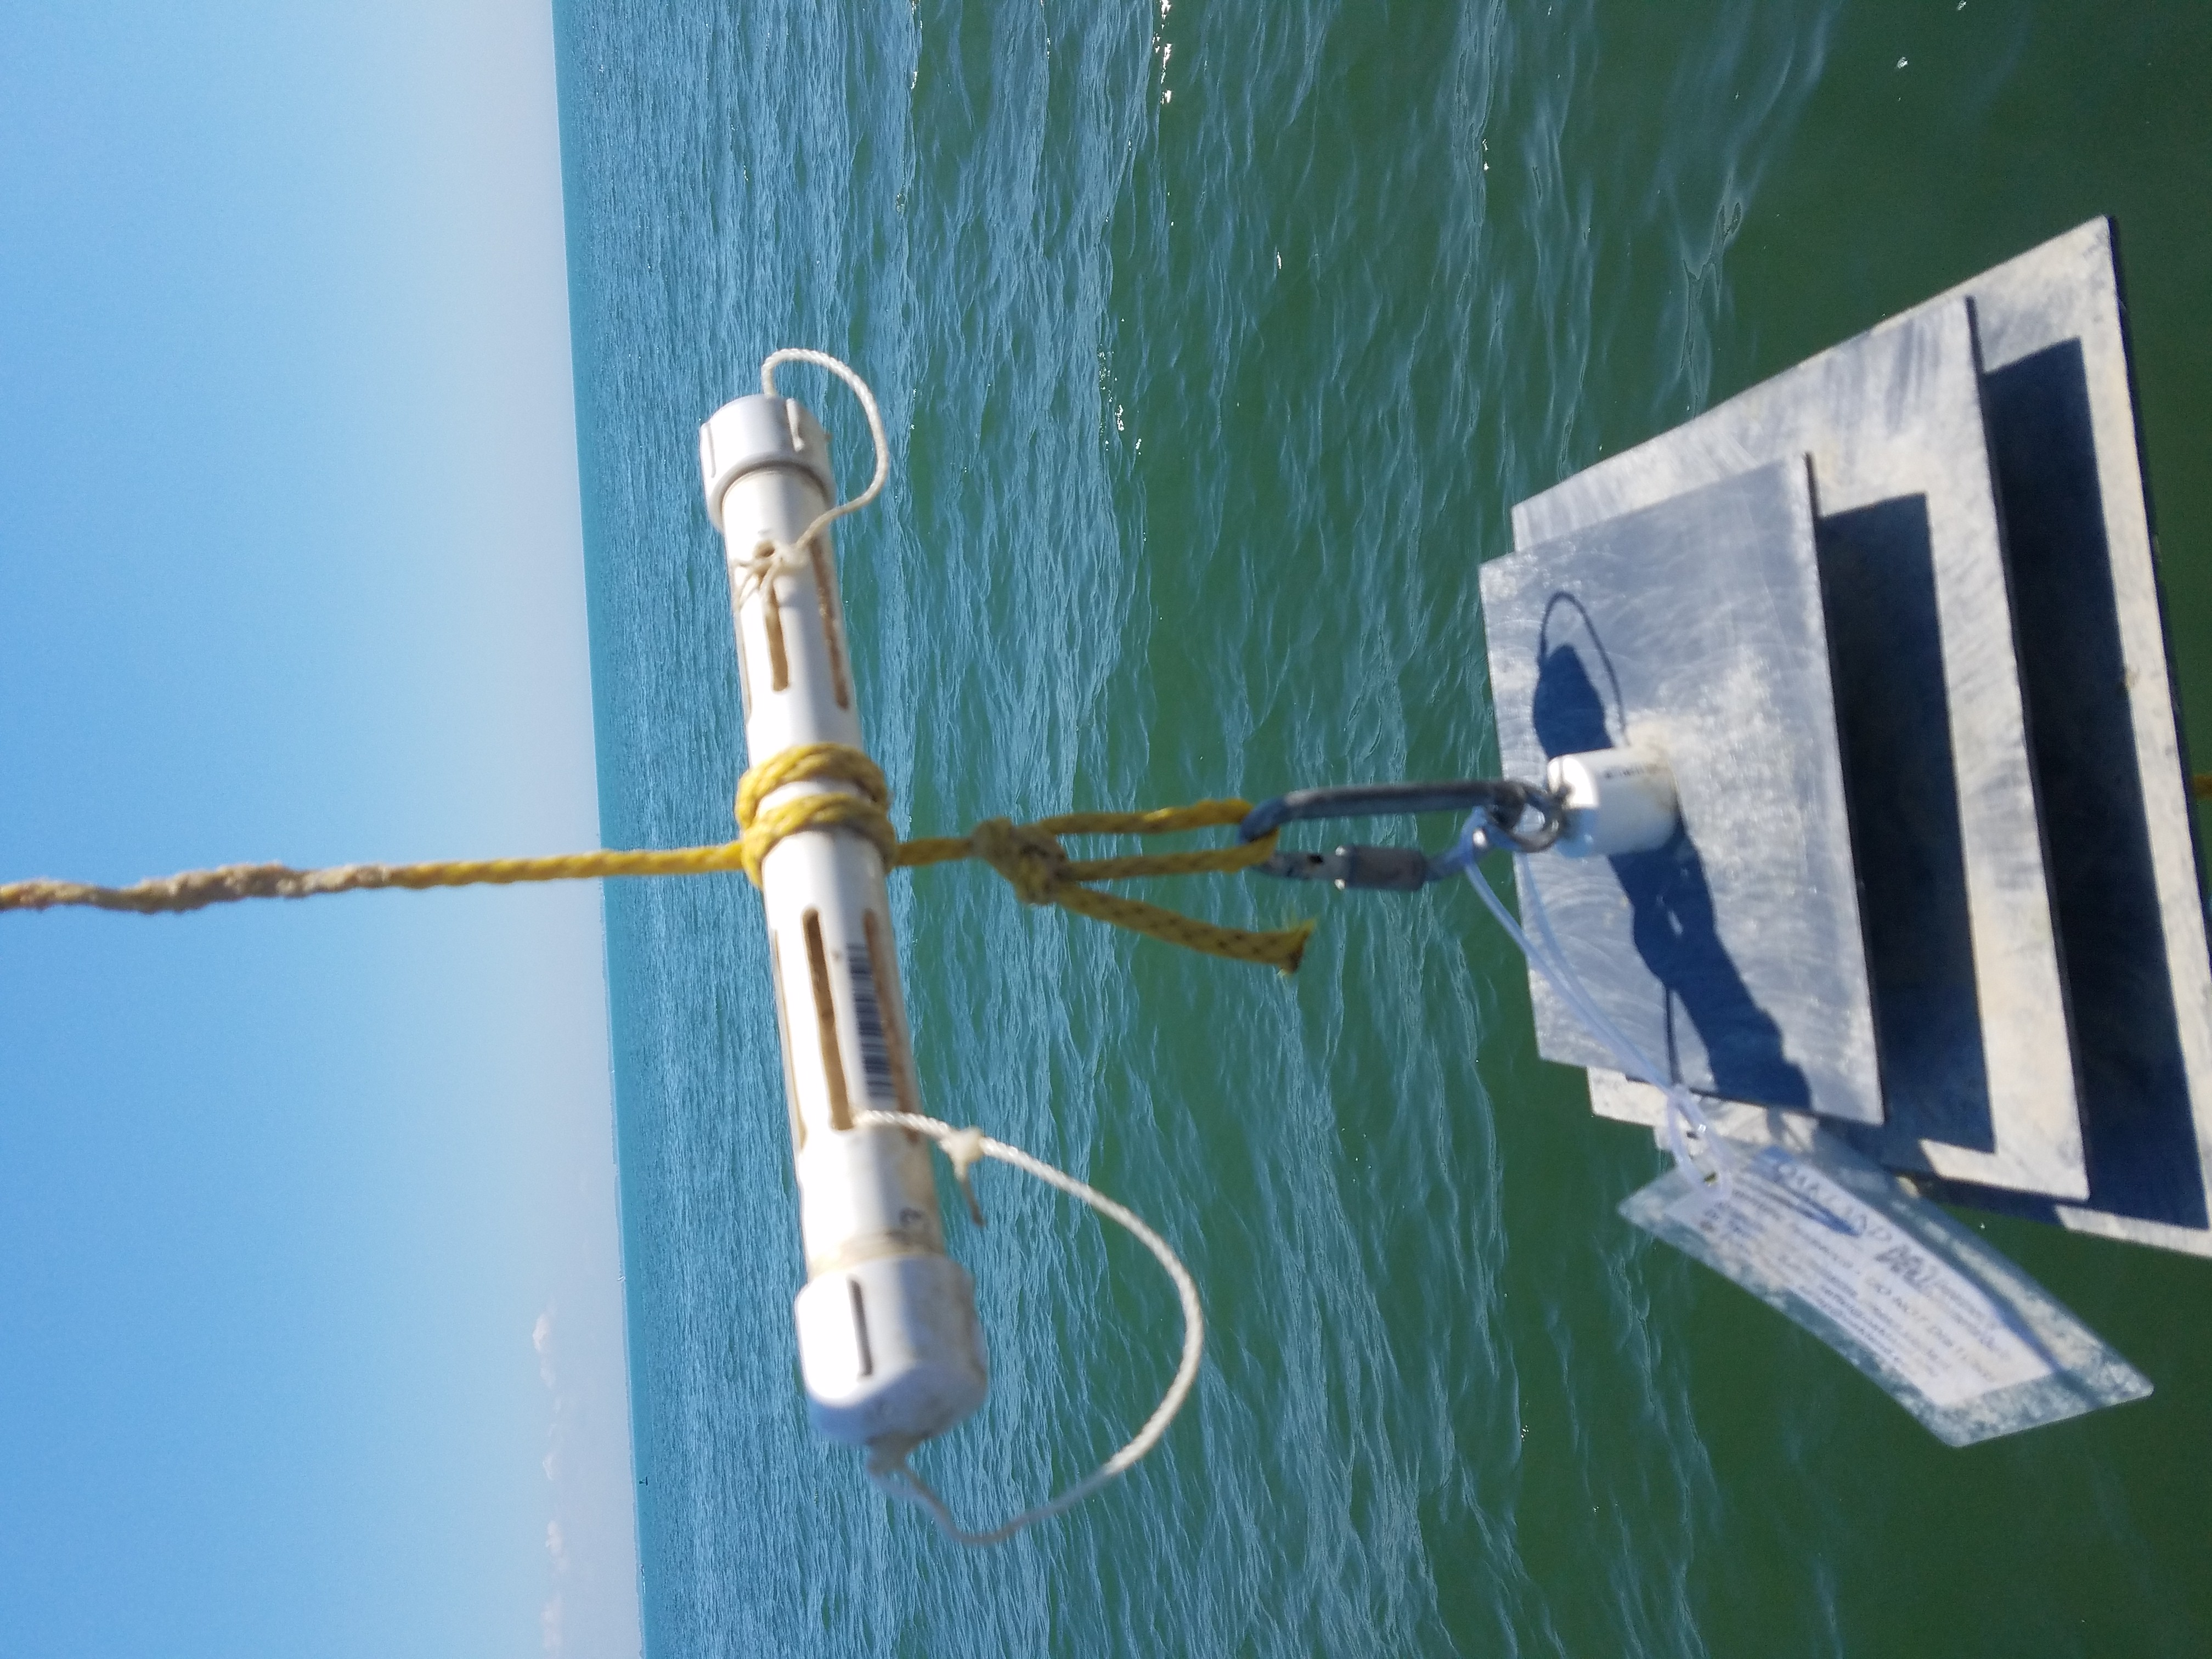
\includegraphics[width=2.3in,angle=-90]{sampler.jpg}
	\end{figure}
\end{columns}


\end{frame}



%%%%%%%%%%%%%%%%%%%%%%%%%%%%%%
\begin{frame}{SPATT}

\begin{columns}
	\column{0.5\textwidth}
	\begin{itemize}
		\item Solid phase adsorbtion toxin tracking 
		\item Dianon HP-20 
		\begin{itemize}
			\item Styrene-divinylbenzene copolymer beads
		\end{itemize} 
		
		\item Sachet filled with resin
		\item Cyanotoxin adsorb onto the resin
		\item Left for one month
	\end{itemize}

	\column{0.5\textwidth}
	\begin{figure}
		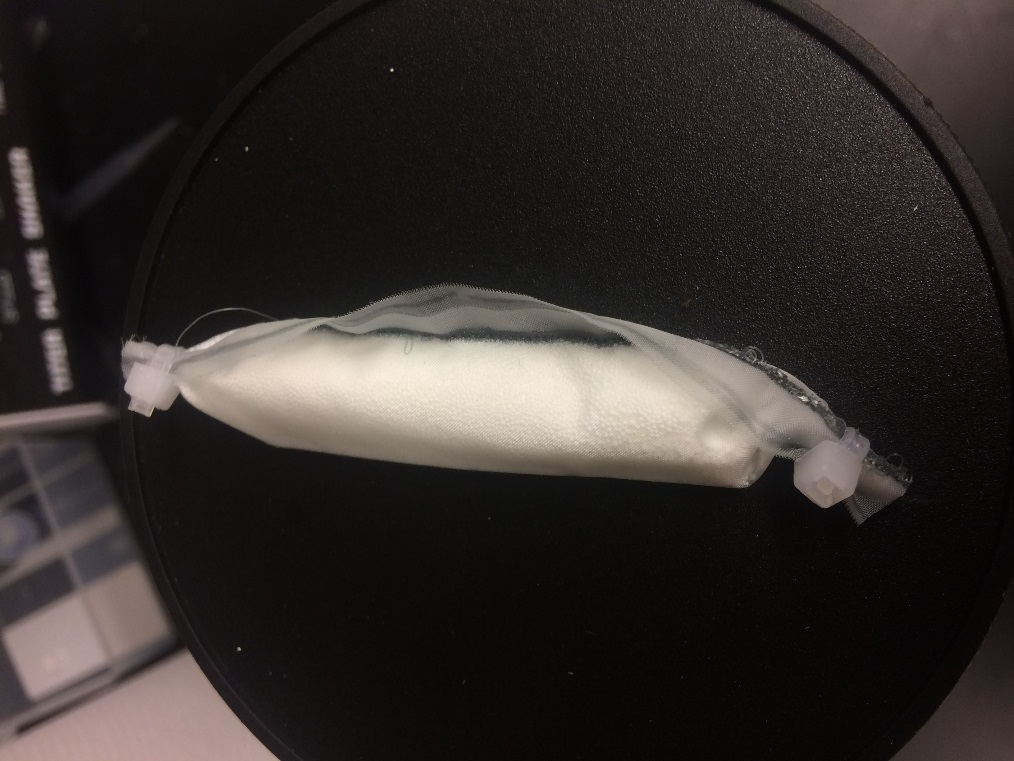
\includegraphics[width=2.3in,angle=-90]{bag.jpg}
	\end{figure}

\end{columns}

\end{frame}

%%%%%%%%%%%%%%%%%%%%%%%%%%%%%

\subsection{Chemical Analysis}

%%%%%%%%%%%%%%%%%%%%%%%%%%%%%%%
\begin{frame}{Nutrients}
	\begin{itemize}
\item Colormetric analysis
\begin{itemize}
		\item Orthophosphorus-P 
		\item Nitrate+nitrite-N 
		\item Ammonia-N 
		\item Total Kejdlahl nitrogen 
		\item Total Phosphorus
	\end{itemize}
\end{itemize}
	

\end{frame}

%%%%%%%%%%%%%%%%%%%%%%%%%%%%%%
\begin{frame}{LC-MS/MS}
	\begin{itemize}
		\item Grab Samples: 
		\begin{itemize}
			\item Freeze/thaw 3x for cell lysis 
			\item Filtered samples with 96 well block 
		\end{itemize}
		\item SPATT: 
		\begin{itemize}
			\item Once retrieved, cyanotoxins are soaked in 85\% methanol with 10mM ammonium formate
		\end{itemize}
		\item Analyzed 12 different microcystin congeners	
	\end{itemize}
	\begin{figure}
		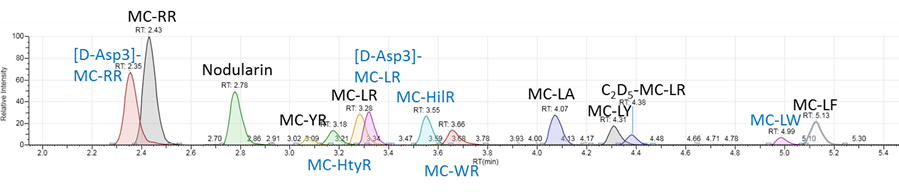
\includegraphics[width=\textwidth]{../figures/LCMS_CONGENERS.png}
	\end{figure}
\end{frame}

%%%%%%%%%%%%%%%%%%%%%%%%%%%%%
\begin{frame}{ELISA}
	\begin{columns}
		\column{0.5\textwidth}
	\begin{itemize}
		\item Enzyme-Linked Immunosorbant Assay
		\item Abraxxis\textsuperscript{a}
		\item Meausures total microcystin
	\end{itemize}
	\column{0.5\textwidth}
	\begin{figure}
		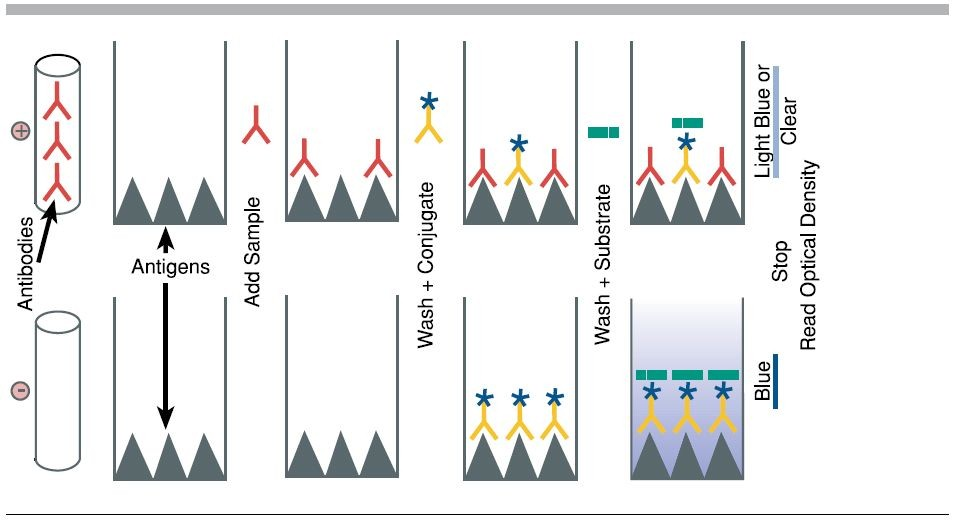
\includegraphics[width=\textwidth]{elisa.jpg}
	\end{figure}
\end{columns}
\footcitetext{[a], noauthor_saxitoxin_nodate}
\end{frame}
\subsection{Statistical Analysis}
%%%%%%%%%%%%%%%%%%%%%%%%%%%%%
\begin{frame}{QPCR}
	\begin{itemize}
		\item Quanitative Polymerase Chain Reaction
		\item Measured target genes:
			\begin{itemize}
				\item \emph{mcyE/ndaF}
				\item \emph{sxtA}
				\item \emph{cyrA}
				\item \emph{16s rRNA}
			\end{itemize}
	\end{itemize}
\end{frame}
%%%%%%%%%%%%%%%%%%%%%%%%%%%%
\begin{frame}{Geospatial Analysis}

	\begin{figure}
		\includegraphics[width=\textwidth]{10.png}
	\end{figure}
\end{frame}

%%%%%%%%%%%%%%%%%%%%%%%%%%%%%
\begin{frame}{Stats}
	\begin{itemize}
		\item Averaged the compiled data by each lake
		\item $log10$ transformed right skewed variables
		\item Program-R \textsuperscript{a}
			\begin{itemize}
				\item Best subset linear regression analyses \textsuperscript{b}
				\item Simple linear regression 
			\end{itemize}
	\end{itemize}
	\footcitetext{r_core_team_r:_2018}
	\footcitetext{miller_leaps:_2017}
\end{frame}
%%%%%%%%%%%%%%%%%%%%%%%%%%%%%
\section{Results}
\subsection{Toxin Results}
\begin{frame}{Cyanotoxins}
	\begin{itemize}
		\item No detection of Cylindrospermopsin or Saxitoxin (gene)
		\item Anatoxin in Brighton Lake (2.80$\mu$g/L) in August 2017
		\item Few instances of microcystin above health advisory from grab samples
			\begin{itemize}
				\item Belleville, Brighton, Cadillac, Ford, Hudson and Wixom Lake
				
			\end{itemize}

			
	\end{itemize}
\end{frame}
%%%%%%%%%%%%%%%%%%%%%%%%%%%%%
\begin{frame}
	\frametitle{Microcystin-ELISA and LC-MS/MS}


	\begin{figure}
		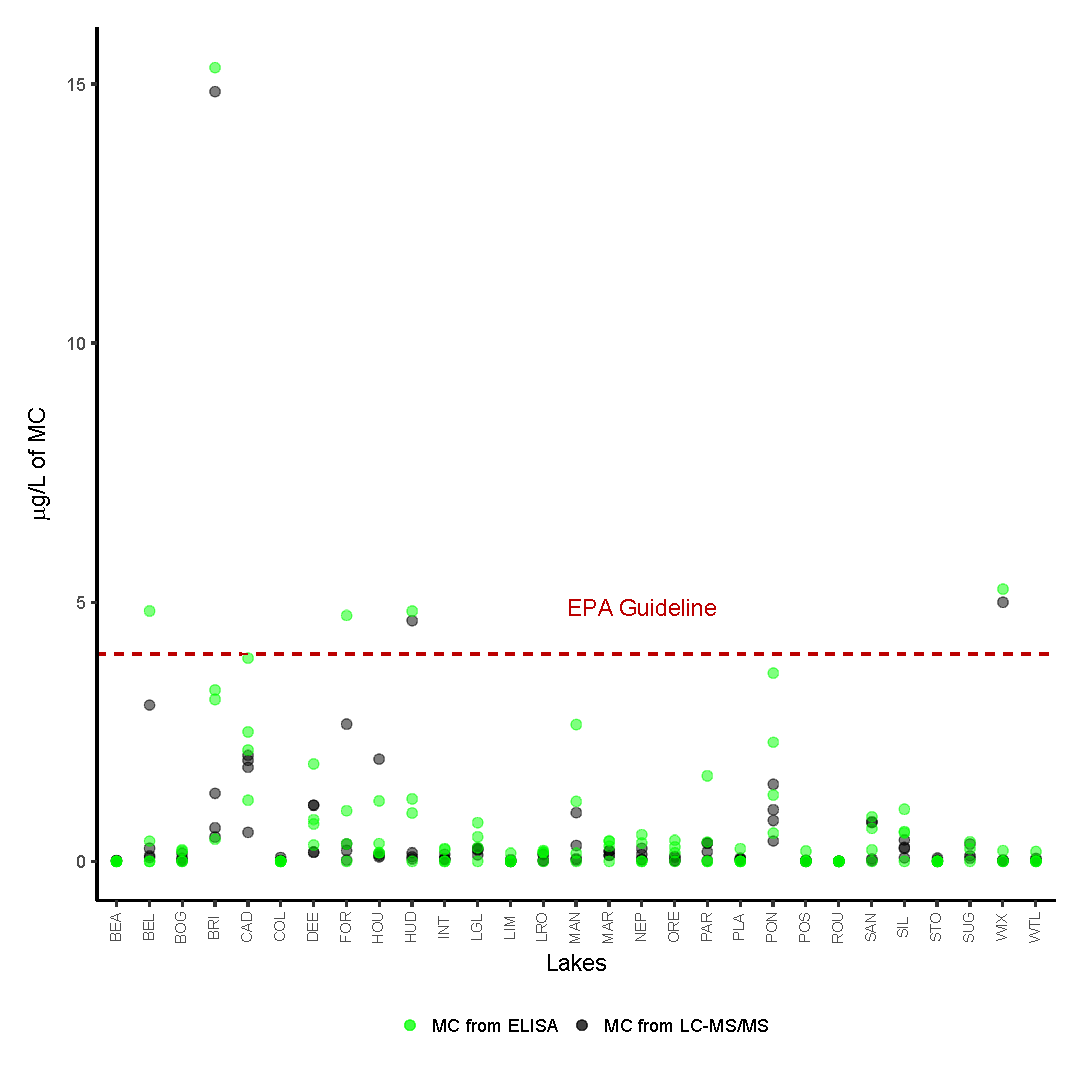
\includegraphics[width=\textwidth,height=0.9\textheight]{../figures/Microcystin.eps}
	\end{figure}

\end{frame}
%%%%%%%%%%%%%%%%%%%%%%%%%%%%%%%%%%%%%%%
\begin{frame}
	\frametitle{Microcystin-LC-MS/MS}


	\begin{figure}
		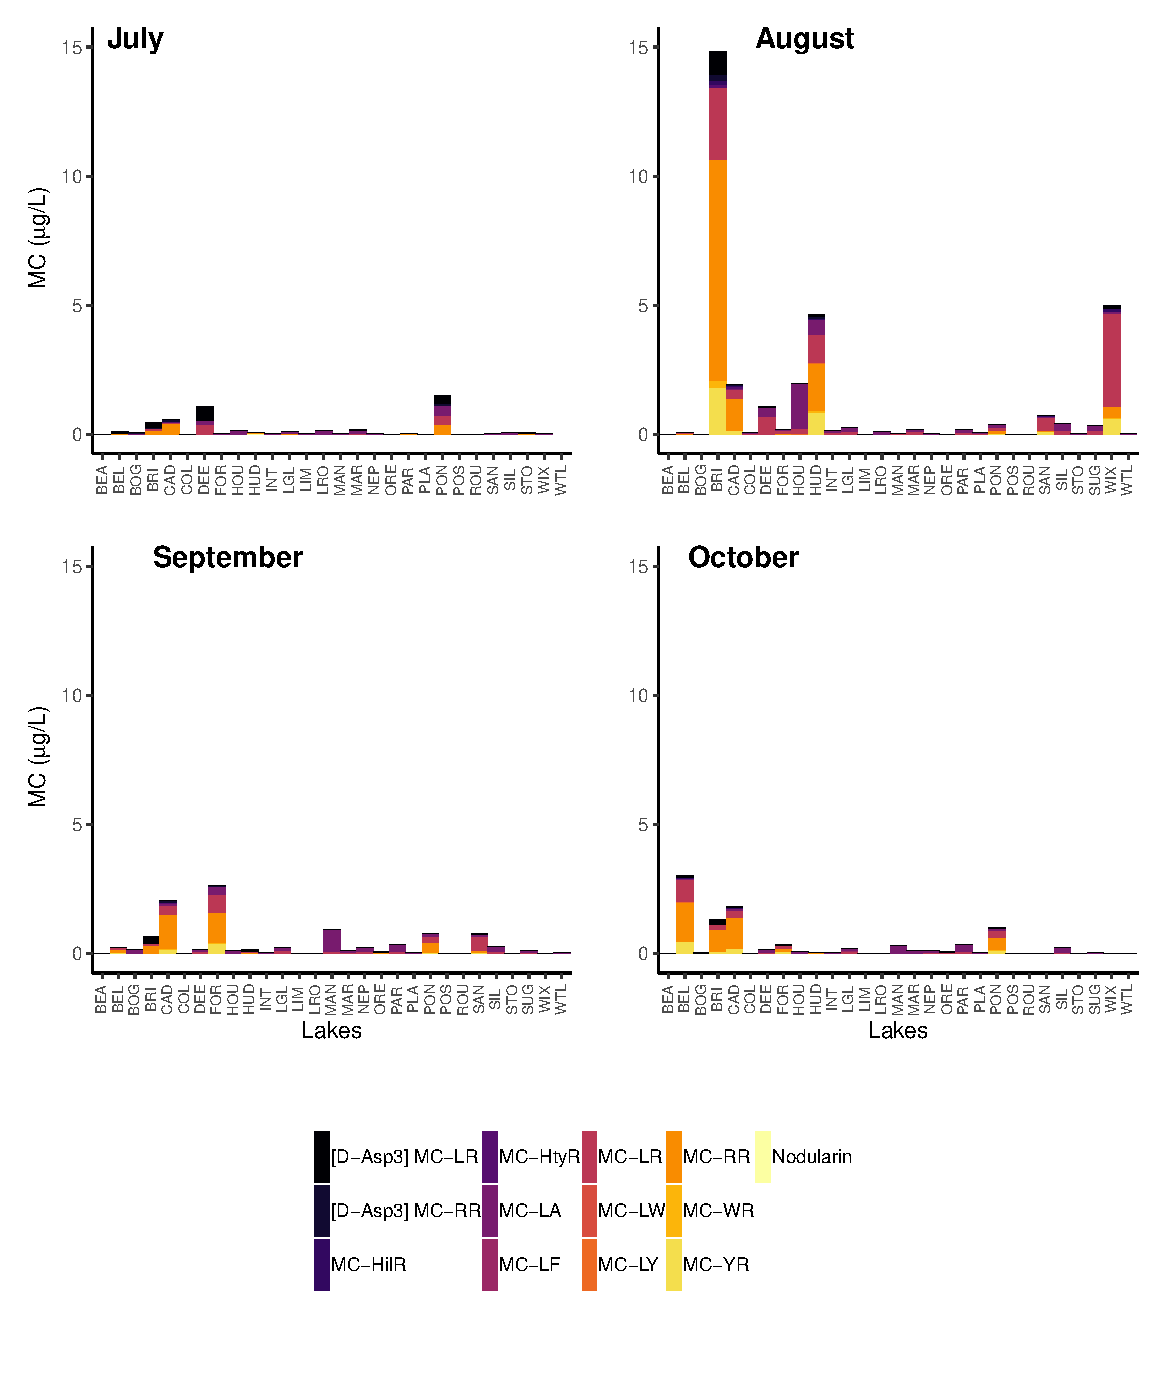
\includegraphics[width=\textwidth,height=0.99\textheight]{1month.eps}
	\end{figure}

\end{frame}

%%%%%%%%%%%%%%%%%%%%%%%%%%%%%%%%%%%%%

%%%%%%%%%%%%%%%%%%%%%%%%%%%%%%%%%%%%%
\begin{frame}
	\frametitle{Microcystin-SPATT}

	\begin{figure}
		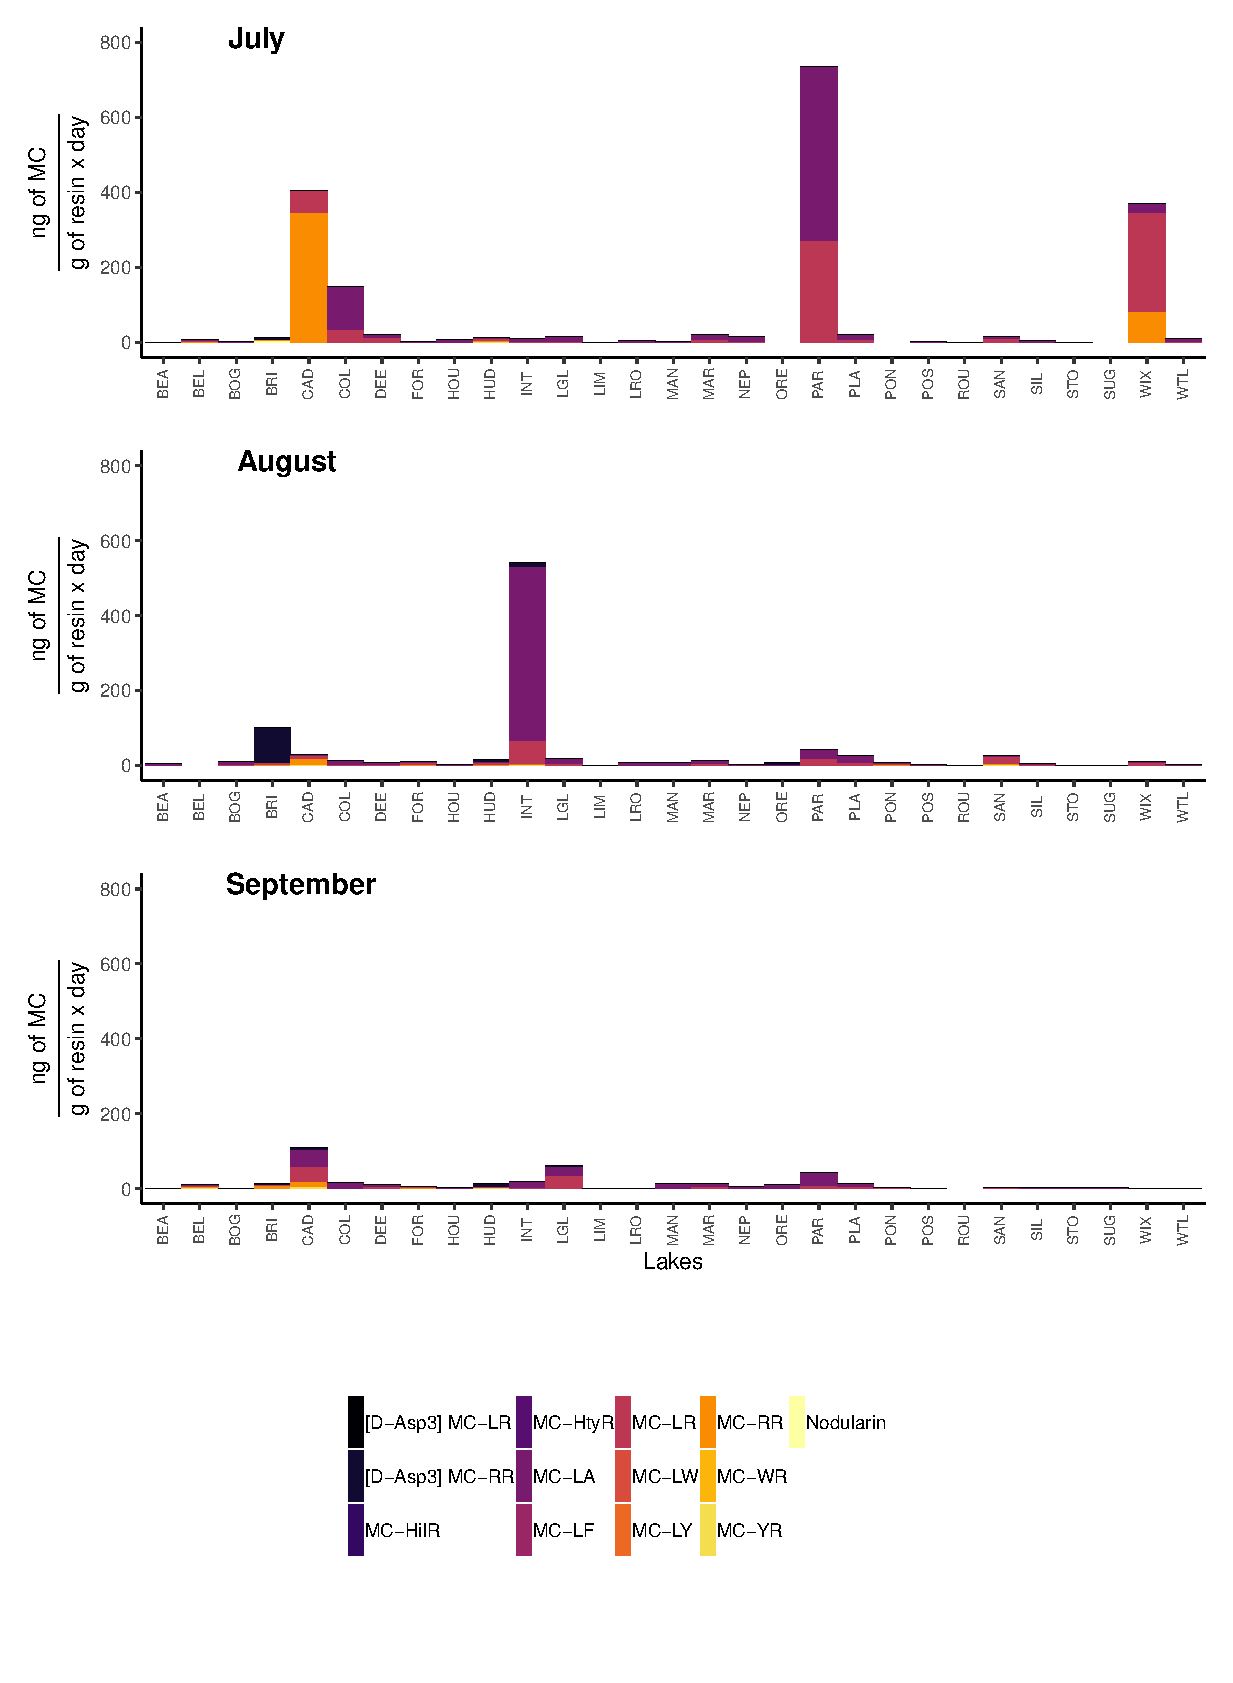
\includegraphics[width=\textwidth,height=1.04\textheight]{1spatter.eps}
	\end{figure}
\end{frame}

%%%%%%%%%%%%%%%%%%%%%%%%%%%%%%%%%%%%%%%
\begin{frame}
	\frametitle{Statistical test}
	\begin{itemize}
		\item Did not find signifigant association between urbanization and harmful algal bloom
		\item QPCR is not an effective tool for detecting cyanotoxins or habs
		\item Turbidity and watershed area was found signifigant
		\item $log10$(turb) ($\beta=0.55$, $F_{{1,27}}=5.90$, $p=0.02$)
		\item $log10$(Watershed Area) ($\beta=0.31$, $F_{{1,27}}=4.88$, $p=0.03$
			\begin{itemize} 
				\item Algae may scatter the light
			\end{itemize}
	\end{itemize}
	\end{frame}


%%%%%%%%%%%%%%%%%%%%%%%%%%%%%%%%%%%%%%%%
	\begin{frame} 
		\frametitle{Turbidity} 
		\begin{figure} 
			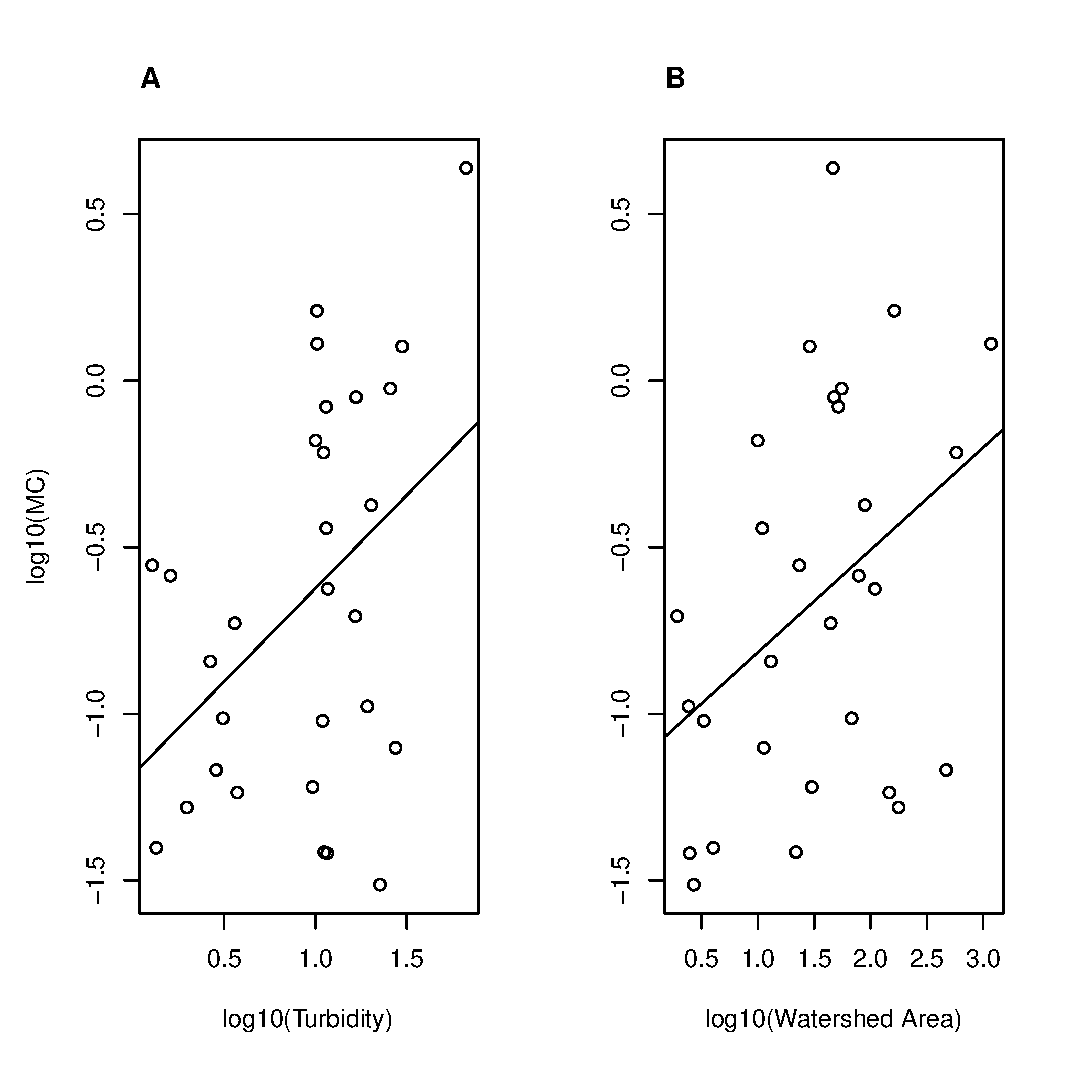
\includegraphics[width=\textwidth, height=0.8\textheight]{../figures/plot2.eps}
		\end{figure}
	\end{frame}

%%%%%%%%%%%%%%%%%%%%%%%%%%%
\section{Conclusion}
\begin{frame}{Conclusion}
	\begin{itemize}
		\item Most of the sampled lakes were low, with a few exceptions 
		\item Did not find any clear environmental drivers 
		\item ELISA and LC-MS/MS agree very well 
		\item Did not find association between urbanization and algal blooms 
		\item Measuring turbidity may provide a preliminary screening tool
	\end{itemize}

	
\end{frame}
%%%%%%%%%%%%%%%%%%%%%%%%%%%%%%%%%%



%%%%%%%%%%%%%%%%%%%%%%%%%%%%%
\begin{frame}{Acknowledgment}

	\begin{itemize} 
		\item My lab team mates: Brian Spies, Andrew Herrpich, Brayden Metcalf, Mikaela Cantu and Alyssa
		\item Jason Sckrabulis, Ryan Mcwhinnie, Melissa Ostrowski, Patrick Long, James Willis
		\item Dr.David Szlag and Dr. Thomas Raffel
		\item Westrick Group at Wayne State University
		\item Ben Southwell at Lake Superiour State University
		\item Michigan Department Environmental Quality
		\item Oakland University and the Chemistry Department
	\end{itemize}
\end{frame}
\begin{frame}
\begin{center}
Thank You
\end{center}
\end{frame}
\section{Appendix}
\begin{frame}
	\frametitle{Appendix1}
	\begin{figure}
	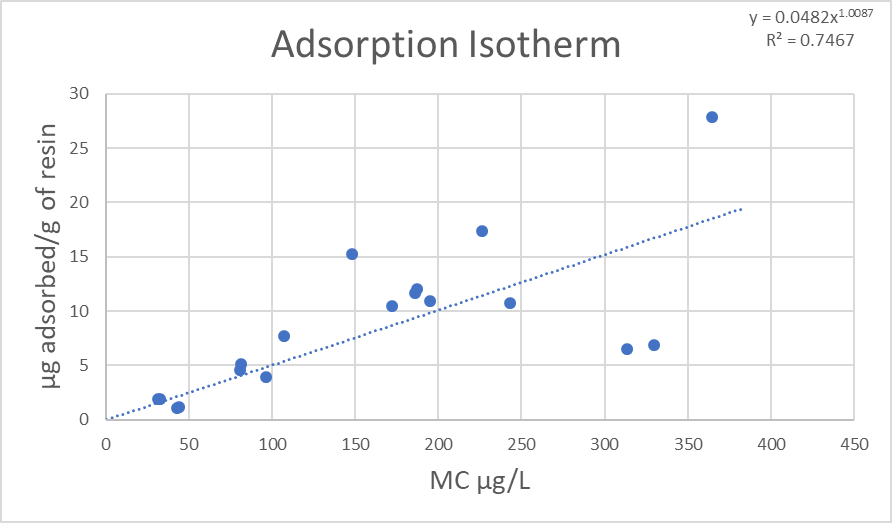
\includegraphics[width=\textwidth]{Isotherm.png}
	\end{figure}	

\end{frame}
%%%%%%%%%%%%%%%%%%%%%%%%%%%%%%%%%%%%%%
\begin{frame}
	\frametitle{Water Chemistry}
	\begin{figure}
		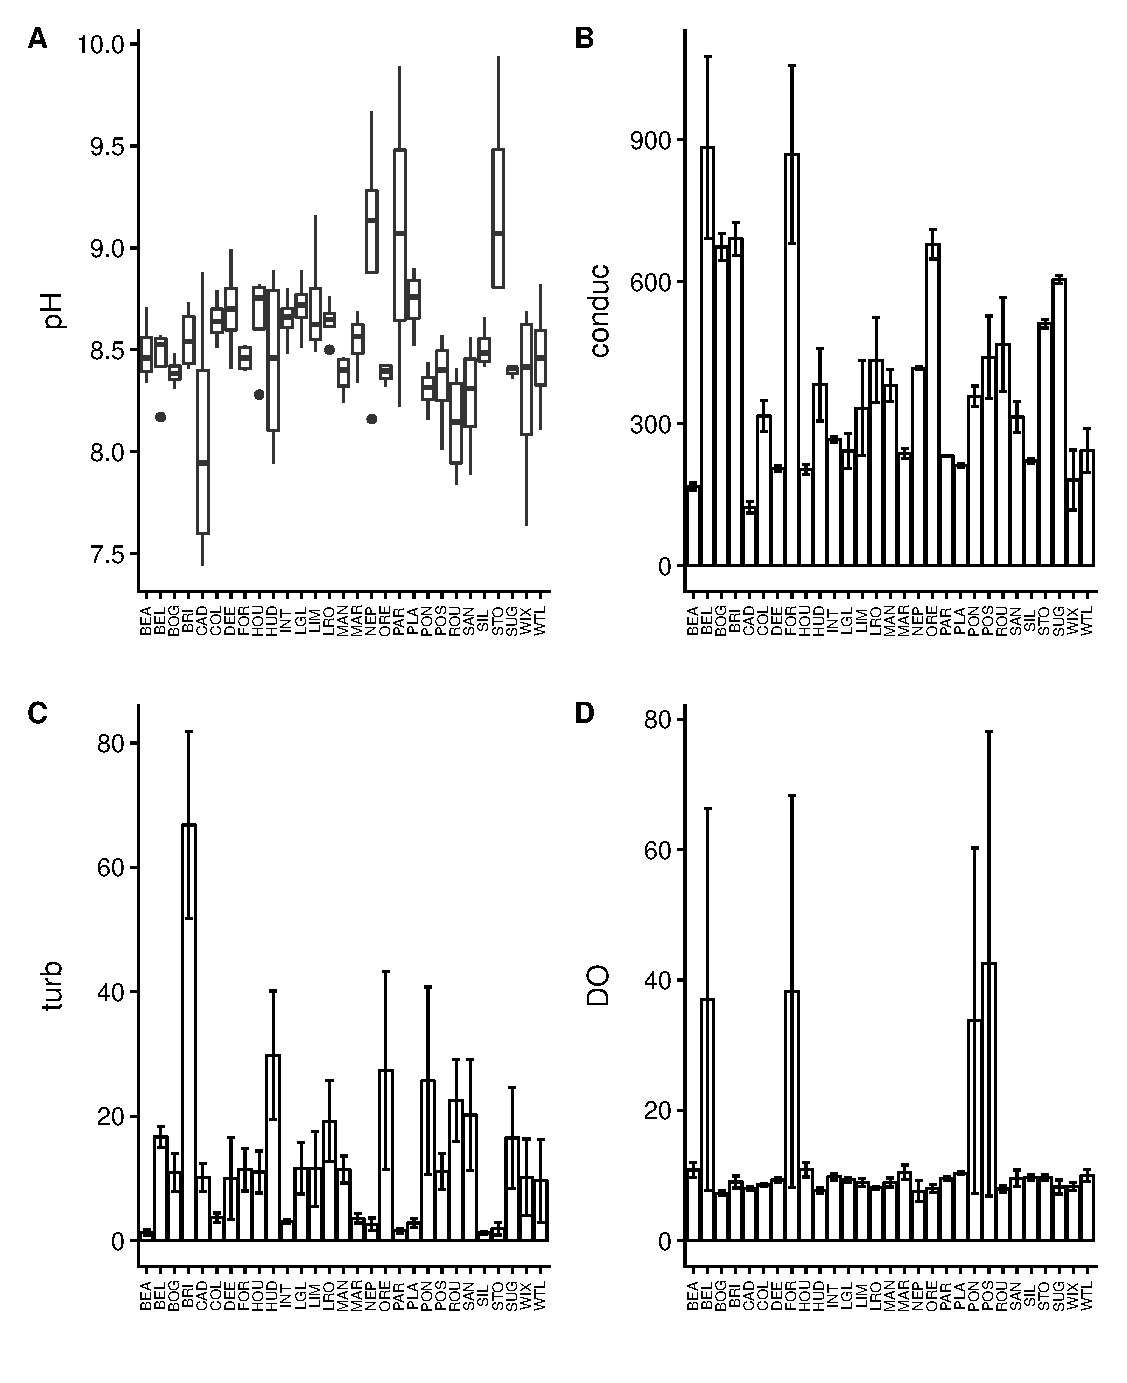
\includegraphics[width=0.7\textwidth,height=\textheight]{../figures/watboxplotlake.eps}
	\end{figure}
\end{frame}
%%%%%%%%%%%%%%%%%%%%%%%%%%%%%%%%%%%%%%%%	
\begin{frame}
	\frametitle{Nutrients}

	\begin{figure}	
		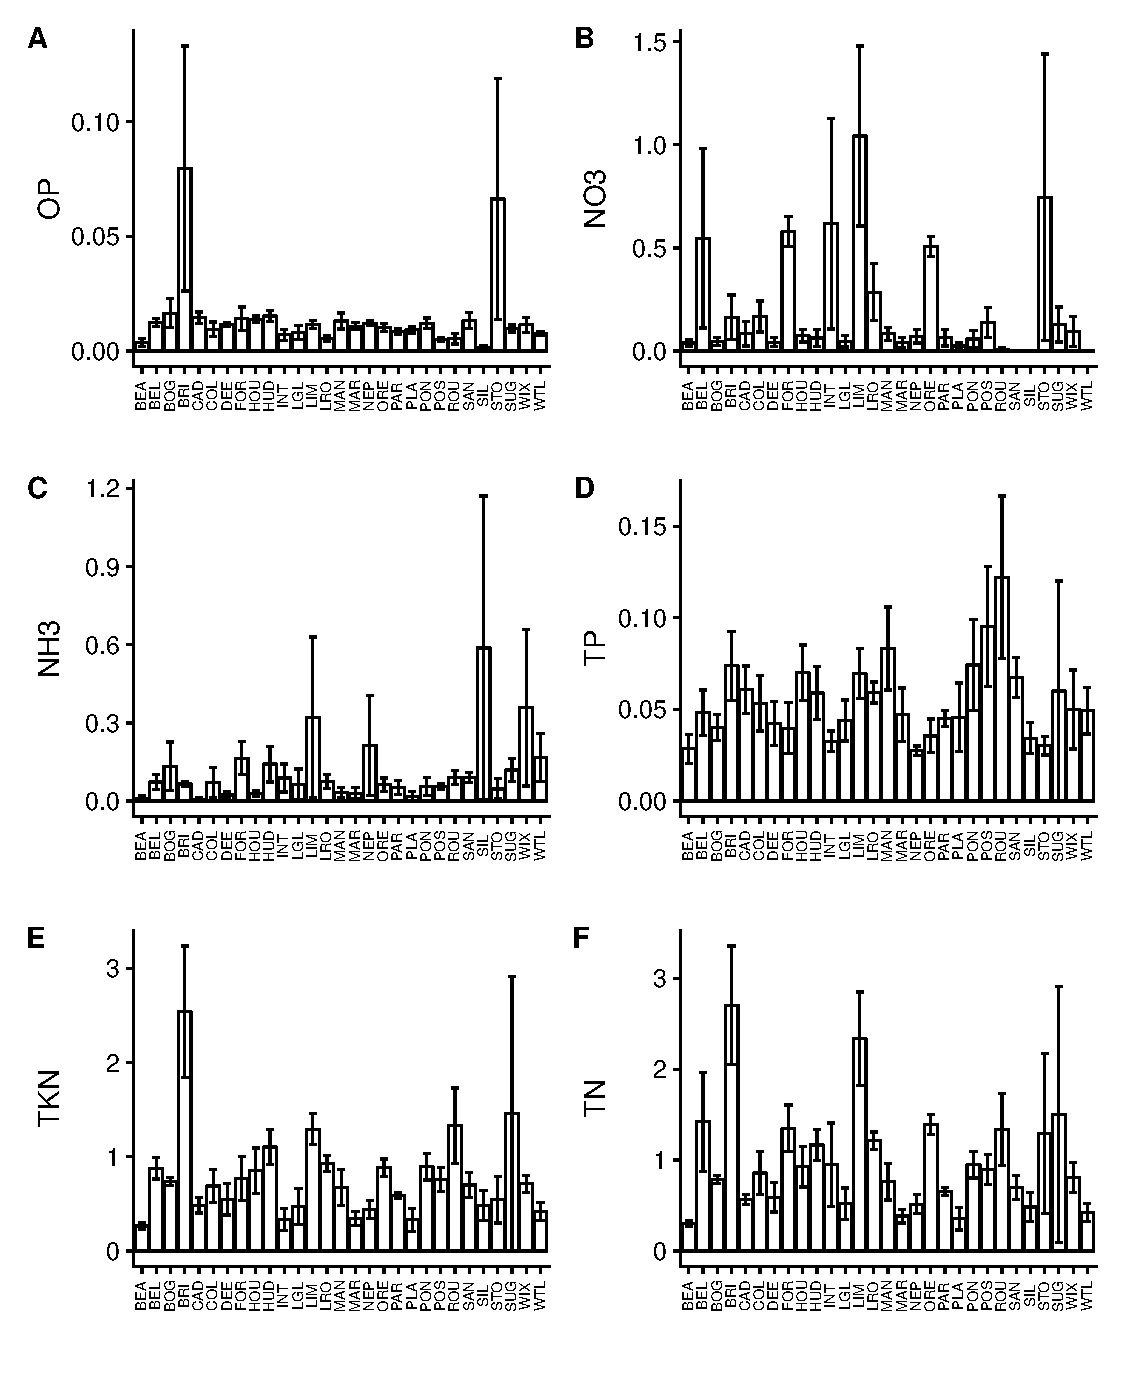
\includegraphics[width=0.7\textwidth, height=\textheight]{../figures/nutboxplotlake.eps}
	\end{figure}

\end{frame}

